\section{Besoins Détaillés}

\subsection{Spécifications Fonctionnelles}

\subsubsection{F1 Utilisateurs}


{\color{orange}{L’application devra permettre de distinguer les différents employés selon le service de la banque auquel ils sont affectés. Il faudra faire attention au fait que cette fédération contient plusieurs banques. Une différentiation au niveau des droits de chaque service devra être faite afin que chaque service puisse échanger des informations avec d’autre service mais garde sa part de confidentialité. Exemple : Le service Ressources Humaines peut envoyer des bilans sur l’effectif total des personnes présentes dans la banque. Le service Ressources Humaines doit pouvoir garder confidentiellement les données concernant le salaire de chaque employé.}}
{\color{green}{L'application permettra de distinguer les employés selon leur rôle: employé, gérant d'une banque ou administrateur de la fédération. Un gérant a la possibilité d'ajouter un nouvel employé ou gérant. L'administrateur de la fédération peut supprimer ou ajouter une banque. La fédération contient plusieurs banques, les
employés et gérants d'une banque ne peuvent pas effectuer d'opération sur les comptes des clients n'appartenant pas à leur banque. Nous avons choisis d'effectuer
cette modification au niveau des rôles pour simplifier l'application. En effet la gestion d'une banque est déjà très complexe, il aurait été difficile pour nous de gérer différents services au sein de chaque banque.}}


\subsubsection{F2 Gestion des comptes client}

Tout les services pourront avoir accès à cette fonctionnalité. Celle-ci devra permettre l’édition de compte à partir desquels nous ferons des virements.Nous pourrons également bloquer et débloquer les comptes. {\color{red}{Cette fonctionnalité permettra également de gérer les prêts des clients, ainsi nous devrons être capable de voir où en est la personne dans ses mensualités, quelle somme il lui reste à rembourser.}} {\color{green}{Nous avons décidé de ne pas gérer les prêts. Nous avons eu un manque de temps et la difficulté de cette fonctionnalité étant semblable à celle des comptes épargne, nous avons jugé peu utile de la créer. Le compte épargne gagne de l'argent tous les mois en fonction d'un taux.}} Il est à noter que la fédération dispose de plusieurs types de compte : compte courant et compte épargne. Il devra également être possible de créer un compte et de le clôturer au moment voulu.

\subsubsection{F3 Envoi de courriels}

Cette fonctionnalité devra permettre l’envoi de courriel au sein de la fédération bancaire.

\subsubsection{F4 Gestion de chèques}

{\color{red}{Cette fonctionnalité devra permettre à chaque service d’effectuer un traitement manuel lors de la réception d’un chèque. La traçabilité est un aspect important de cette fonctionnalité. Ainsi on devra pouvoir savoir de qui vient le chèque et la date à laquelle il a été déposé ainsi que l’employé qui a traité la demande.}}
{\color{green}{Cette fonctionnalité étant similaire à la fonctionnalité permettant de faire de virements, nous avons décidé de ne pas l'implémenter car nous manquions de temps.}}

\subsubsection{F5 Statistiques}

{\color{orange}{Cette fonctionnalité sera accessible à tous les services de chaque banque. Elle devra permettre de suivre le nombre de dépôts de chèques, le nombre de virements à effectuer et la valeur totale du flux monétaire journalier ayant transité.}}
{\color{green}{Nous avons fait des statistiques mais pas celles annoncées, nous avons calculé le nombre de clients de la fédération, le nombre d'opérations effectuées, le nombre de comptes courants et épargnes des banques de la fédération.}}


\subsubsection{F6 Gestion de prêt}

{\color{red}{Cette fonctionnalité devra permettre de mettre à jour en temps réel les différents comptes bancaires vis-à-vis de leurs prêts bancaires.}} {\color{green}{Comme expliqué précédemment, la fonctionnalité de gestion de prêt bancaires n'a pas été implémentée à cause d'un manque de temps et du fait que sa gestion soit similaire à une autre fonctionnalité implémentée}}

\subsection{Constitution des Lots}

\subsubsection{Lot 1}

Ce premier lot à délivrer pour le 21 mars 2016 devra permettre la mise en place de la base de données. La fonctionnalité F1 devra également être terminée.

\subsubsection{Lot 2}

Ce lot à délivrer pour le 11 avril 2016 devra implémenter la fonctionnalité F2 en plus des fonctionnalités développées dans le lot précédent.


\subsubsection{Lot 3}

Ce lot à délivrer pour le 11 mai 2016 devra implémenter les fonctionnalités F3{\color{red}{, F4}}, F5 {\color{red}{et F6}} en plus des fonctionnalités développées dans le lot précédent.

\subsection{Diagramme de Cas d'Utilisation}

\begin{figure}[!h]
\begin{center}

   \caption{\label{} Diagramme de Cas d'Utilisation}
   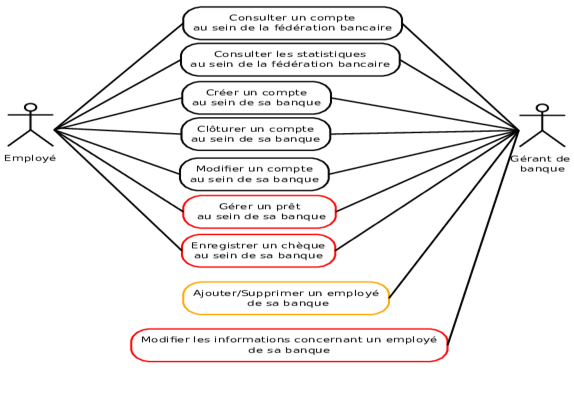
\includegraphics[scale=0.65]{images/CasUtilisation2.png}
   \centering

\end{center}
\end{figure}

\subsection{Spécifications d'Interface}
La maquette en annexe présente approximativement le résultat visuel que devra fournir l’application.

\subsection{Spécifications Opérationnelles}

\subsubsection{Performances}

L’application devra être performante sous deux systèmes d’exploitation : Linux et Windows. L’application devra supporter d’être utilisée par plusieurs utilisateurs simultanément. {\color{orange}{Ces utilisateurs ne pourront pas accéder au même compte en banque en même temps mais pourront effectuer des manipulations sur des comptes différents en même temps.}}{\color{green}{Les utilisateurs peuvent accéder au même compte en même temps et effectuer des opérations}} Les transactions effectuées sur les comptes tels que par exemple un virement d’argent ou le blocage d’un compte devront avoir un temps de réponse inférieur à une seconde.

\subsubsection{Sécurité, Intégrité et Sûreté}

Tous les utilisateurs de l’application n’auront pas accès à toutes les données. La restriction de leur accès dépendra de leur rôle et de la banque dans laquelle ils travaillent. Les employés d’une banque pourront consulter les comptes et les statistiques des clients d’une autre banque mais ne pourront pas éditer leur compte. Au sein d’une même banque, nous distinguerons deux rôles : les gérants de banque et les employés. Les gérants de banque auront les mêmes accès que les employés et pourront en plus gérer les employés (ajouter {\color{red}{ou supprimer des employés, modifier leur salaire}}).Lors de la connexion, il sera demandé à l’utilisateur d’entrer {\color{orange}{son nom, sa banque et son mot de passe.}} {\color{green}{L'utilisateur a uniquement besoin d'entrer son identifiant et son mot de passe.}} {\color{orange}{Grâce à son nom et sa banque, il sera possible de retrouver son rôle afin d’appliquer les restrictions nécessaires.}}{\color{green}{Grâce à son identifiant, il sera possible de retrouver sa banque et son rôle afin d'appliquer les restrictions nécessaires}}

\subsubsection{Base de Données}

Pour notre projet, nous avons besoin d’une base de données.
Cette base de données stockera tous les noms des clients des différentes banques,
leurs adresses mail afin de pouvoir les avertir automatiquement, l’argent dont ils disposent sur leurs comptes,
{\color{red}{leurs prêts en cours}}{\color{green}{La fonctionnalité de gestion des prêts n'a pas été implémentée}}
et un indicateur permettant de bloquer/débloquer leurs comptes. La base contiendra également le rôle de chaque employé
de chaque banque afin de pouvoir connaître les restrictions à appliquer à son compte. {\color{red}{La base va aussi nous
permettre de stocker différentes données comme par exemple le nombre de virements effectués ou le nombre de chèques
déposés pour pouvoir par la suite réaliser des statistiques.}}
{\color{green}{La base contient la liste des opérations effectuées. À partir de cette liste, il est donc possible de connaître le nombre d'opérations grâce à une simple requête.}}


\section{{\color{orange}{Annexes}}}


{\color{green}{Pour les vues, nous avons remplacé les maquettes par les vues que nous avons réellement créé.}}

\subsection{Vue de connexion}

\begin{figure}[H]
\begin{center}

   \caption{\label{} Formulaire de connexion pour le personnel}
   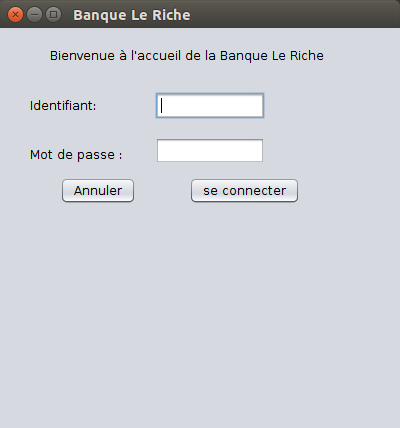
\includegraphics[scale=0.4]{images/connexion.png}
   \centering
 \end{center}
\end{figure}


\subsection{Vues de l'administrateur}

\begin{figure}[H]
\begin{center}

   \caption{\label{} Menu de l'administrateur}
   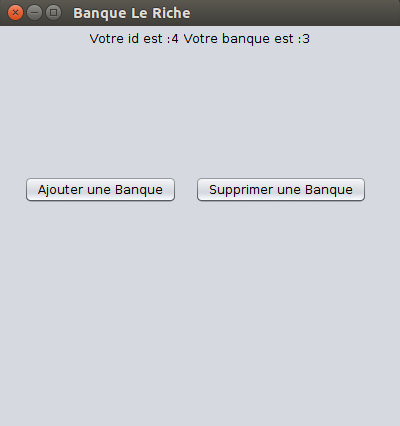
\includegraphics[scale=0.4]{images/adminMenu.png}
   \centering

\end{center}
\end{figure}

\begin{figure}[H]
\begin{center}

   \caption{\label{} Formulaire ajouter banque, disponible uniquement pour l'administrateur}
   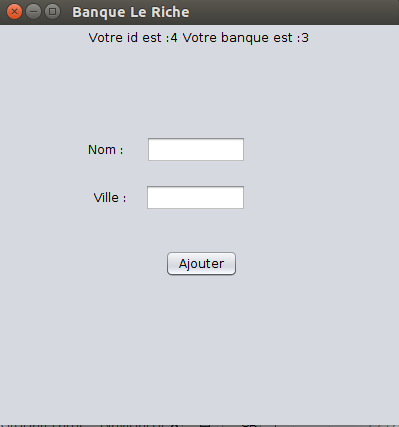
\includegraphics[scale=0.4]{images/AjouterBanque.png}
   \centering
 \end{center}
\end{figure}

 \subsection{Vues de des Gérants et des Employés}

\begin{figure}[H]
\begin{center}

   \caption{\label{} Menu principal}
   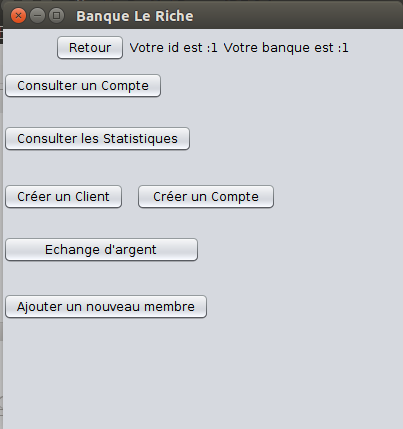
\includegraphics[scale=0.4]{images/gererComptes.png}
   \centering
 \end{center}
\end{figure}

\begin{figure}[H]
\begin{center}

   \caption{\label{} Consulter le ou les comptes d'un client}
   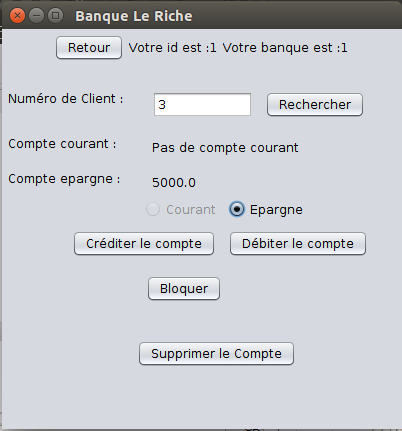
\includegraphics[scale=0.4]{images/ConsulterCompte.png}
   \centering
 \end{center}
\end{figure}

\begin{figure}[H]
\begin{center}

   \caption{\label{} Consulter les statistiques de la fédération}
   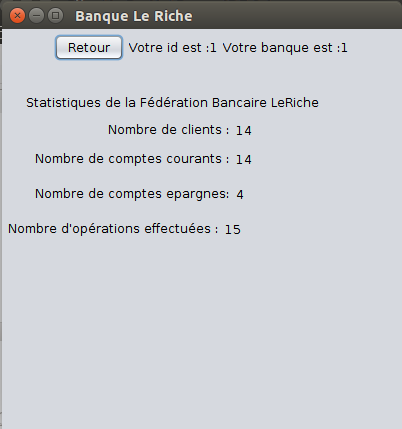
\includegraphics[scale=0.4]{images/Stats.png}
   \centering
 \end{center}
\end{figure}

\begin{figure}[H]
\begin{center}

   \caption{\label{} Formulaire de création d'un client et de son compte}
   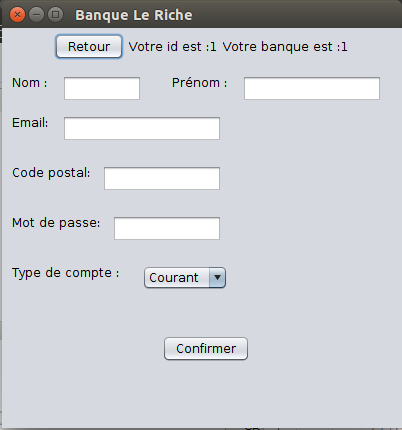
\includegraphics[scale=0.4]{images/creerClient.png}
   \centering
 \end{center}
\end{figure}

\begin{figure}[H]
\begin{center}

   \caption{\label{} Formulaire de création d'un compte associé à un client déjà existant}
   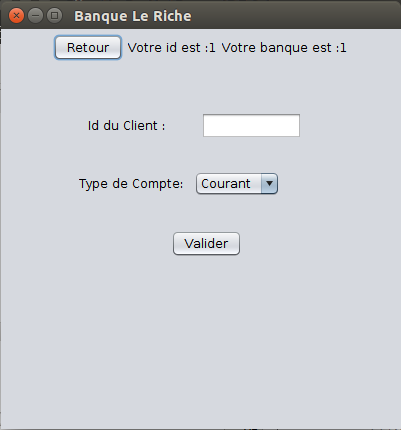
\includegraphics[scale=0.4]{images/CreerCompte.png}
   \centering
 \end{center}
\end{figure}

\begin{figure}[H]
\begin{center}

   \caption{\label{} Effectuer un virement entre deux comptes}
   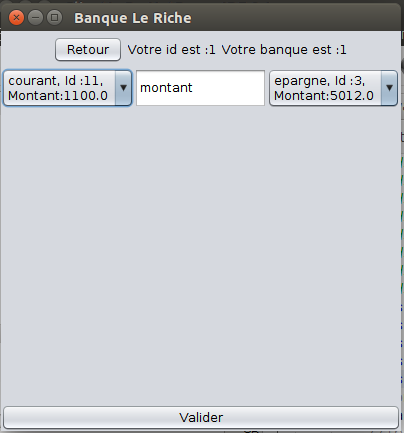
\includegraphics[scale=0.4]{images/EchangeArgent.png}
   \centering
 \end{center}
\end{figure}


\subsection{Vue uniquement visible par les Gérants}

\begin{figure}[H]
\begin{center}

   \caption{\label{} Formulaire de création d'un nouveau membre du personnel}
   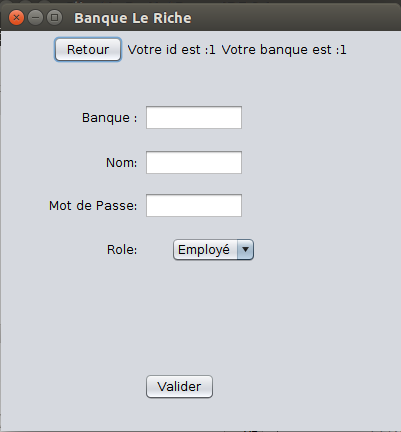
\includegraphics[scale=0.4]{images/CreerPersonnel.png}
   \centering
 \end{center}
\end{figure}
